\documentclass{beamer}

%% \documentclass[handout]{beamer}
%% % use this with the [handout] option to create handouts for the audience
%% \usepackage{pgfpages}
%% \pgfpagesuselayout{2 on 1}[a4paper,border shrink=5mm]

\mode<presentation>
{
  \usetheme{Diku}
% set this to your preferences:
  \setbeamercovered{invisible}
%  \setbeamercovered{transparent}
}

\usepackage{graphicx}
\usepackage{epic}

\usepackage{amsmath}
\usepackage{amssymb}
\usepackage{amsthm}

\newcommand{\basetop}[1]{\vtop{\vskip-1ex\hbox{#1}}}
\newcommand{\source}[1]{\let\thefootnote\relax\footnotetext{\scriptsize\textcolor{kugray1}{Source: #1}}}

% for coloured code citation in text:
\usepackage{fancyvrb}

%%%%%%%%%%%%%%%%%%%%%%%%%%%%%%%%%
%%%%%    code sections   %%%%%%%%
%%%%%%%%%%%%%%%%%%%%%%%%%%%%%%%%%

% code highlighting commands in own block
\DefineVerbatimEnvironment{code}{Verbatim}{fontsize=\scriptsize}
\DefineVerbatimEnvironment{icode}{Verbatim}{fontsize=\scriptsize}

% Fancy code with color commands:
\DefineVerbatimEnvironment{colorcode}%
        {Verbatim}{fontsize=\scriptsize,commandchars=\\\{\}}

%%%%%%%%%%%%%%%%%%%%%%%%%%%%%%%%%%
%%%%%    some coloring    %%%%%%%%

\definecolor{Red}{RGB}{220,50,10}
\definecolor{Blue}{RGB}{0,51,102}
\definecolor{Yellow}{RGB}{102,51,0}
\definecolor{Orange}{RGB}{178,36,36}
\definecolor{Grey}{RGB}{180,180,180}
\definecolor{Green}{RGB}{20,120,20}
\definecolor{Purple}{RGB}{160,50,100}
\newcommand{\red}[1]{\textcolor{Red}{{#1}}}
\newcommand{\blue}[1]{\textcolor{Blue}{{#1}}}
\newcommand{\yellow}[1]{\textcolor{Yellow}{{#1}}}
\newcommand{\orange}[1]{\textcolor{Orange}{{#1}}}
\newcommand{\grey}[1]{\textcolor{Grey}{{#1}}}
\newcommand{\green}[1]{\textcolor{Green}{{#1}}}
\newcommand{\purple}[1]{\textcolor{Purple}{{#1}}}




% use "DIKU green" from our color theme for \emph
\renewcommand{\emph}[1]{\textcolor{structure}{#1}}
% use some not-too-bright red for an \emp command
\definecolor{DikuRed}{RGB}{130,50,32}
\newcommand{\emp}[1]{\textcolor{DikuRed}{ #1}}
\definecolor{CosGreen}{RGB}{10,100,70}
\newcommand{\emphh}[1]{\textcolor{CosGreen}{ #1}}
\definecolor{CosBlue}{RGB}{55,111,122}
\newcommand{\emphb}[1]{\textcolor{CosBlue}{ #1}}
\definecolor{CosRed}{RGB}{253,1,1}
\newcommand{\empr}[1]{\textcolor{CosRed}{ #1}}

\newcommand{\mymath}[1]{$ #1 $}
\newcommand{\myindx}[1]{_{#1}}
\newcommand{\myindu}[1]{^{#1}}

\newcommand{\Fasto}{\textsc{Fasto}\xspace}


%%%%%%%%%%%%%%%%%%%%

\title[Type Checking]{Type Checking}

\author[C.~Oancea]{Cosmin E. Oancea\\{\tt cosmin.oancea@diku.dk}}

\institute{Department of Computer Science (DIKU)\\University of Copenhagen}


\date[December 2012]{December 2012 Compiler Lecture Notes}


\begin{document}

\titleslide

\input{Struct_Interm/StructTC}

\begin{frame}[fragile]
	\tableofcontents
\end{frame}


%%%%%%%%%%%%%%%%%%%%%%%%%%%%%%%%%%%%%%%%%%%%%%%%%%%%%%%%%%%%%%%%%%%%%%
%%%%%%%%%%%%%%%%%%%%%%%%%%%%%%%%%%%%%%%%%%%%%%%%%%%%%%%%%%%%%%%%%%%%%%
\section{Interpretation Recap: Synthesized/Inherited Attributes}

\begin{frame}[fragile,t]
   \frametitle{Interpretation Recap}

\begin{block}{$~~~~~~~~~~~~~$ Compiler $~~~~~~~~~~~~~$ {\em vs.} $~~~~~~~~~~~~~~$ Interpreter}
\begin{columns}
\column{0.31\textwidth}
\begin{tabular}{c}
{\em source program}\\
$\downarrow$\\
\framebox{\emph{Compiler}}\\
$\downarrow$\\
{\em target program}
\end{tabular}
\column{0.31\textwidth}
\begin{tabular}{c}
{\em input}\\
$\downarrow$\\
\framebox{Target Program}\\
$\downarrow$\\
{\em output}
\end{tabular}
\column{0.31\textwidth}
\begin{tabular}{c}
{\em source}$~~~~~~~~~~~$\\
{\em program}$~~~${\em input}\\
$\downarrow~~~~~~~\downarrow$\\
\framebox{\emp{Interpreter}}\\
$\downarrow$\\
{\em output}
\end{tabular}
\end{columns}
\end{block}

{\em The interpreter} directly {\em executes} one by one the operations specified
in the {\em source program} on the {\em input} supplied by the user, by using the
facilities of its implementation language.

\bigskip

{\em Why interpret?} Debugging, Prototype-Language Implementation, etc.

\end{frame}




\begin{frame}[fragile,t]
   \frametitle{Synthesized {\em vs} Inherited Attributes}

\bigskip

A compiler phase consists of one or several traversals of the \textsc{AbSyn}.
We formalize it via {\em attributes}:

\bigskip

\begin{description}

    \item[Inherited:] info passed downwards on the \textsc{AbSyn} traversal, i.e.,
                        from root to leaves. Think: helper structs. \alert{Example?}\bigskip

    \item[Synthesized:] info passed upwards in the \textsc{AbSyn} traversal, i.e., from
                        leaves to the root. Think: the result. \alert{Example?}\bigskip

    \item[Both:]    Information may be synthesized from one subtree and
                    may be inherited/used in another subtree (or at a latter
                    parse of the same subtree). \alert{Example?}

\end{description}

\end{frame}


\begin{frame}[fragile,t]
   \frametitle{Example of Inherited Attributes}

The variable and function symbol tables, i.e., \emp{{\em vtable}} and \emp{{\em ftable}}, 
in the interpretation of an expression: 

\bigskip

$Eval_{Exp} (Exp, vtable, ftable ) = ...$

\bigskip

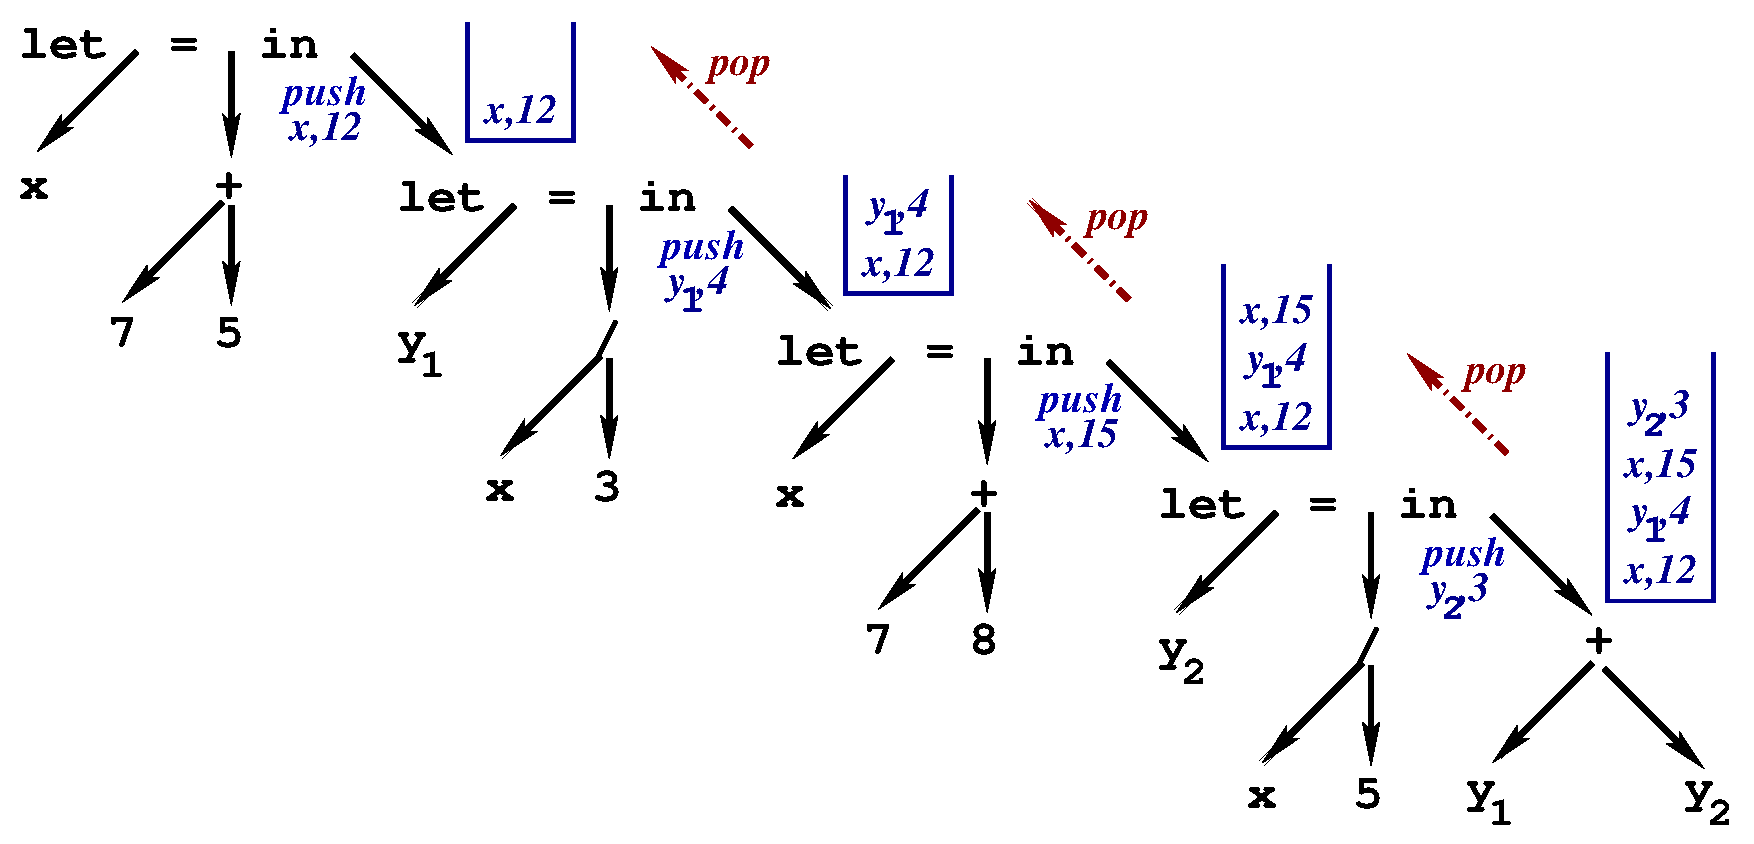
\includegraphics[width=65ex]{Figures/ExpIntStack}

\end{frame}


\begin{frame}[fragile,t]
   \frametitle{Example of Synthesized Attributes}

\bigskip
\bigskip

The interpreted value of an expression / program is synthesized.

\bigskip
\bigskip

Example of both {\em synthesized} and {\em inherited} attributes:

\bigskip

\emp{$~~~~vtable = Bind_{TypeIds} (TypeIds, args)$} 

\smallskip

\emp{$~~~~ftable = Build_{ftable} (Funs)$}

\bigskip

and used in the interpretation of an expression.
\end{frame}


\begin{frame}[fragile,t]
   \frametitle{Interpretation {\em vs} Compilation Pros and Cons}

%\bigskip

\noindent\begin{itemize}
\item[$+$] Simple (good for impatient people).\bigskip

\item[$+$] Allows easy modification / inspection of the program at run time.\bigskip

\item[$-$] Typically, it does not discover all type errors. \alert{Example?}\bigskip

\item[$-$] Inefficient execution: \smallskip
        \begin{itemize}
            \item Inspects the \textsc{AbSyn} repeatedly, e.g., symbol table lookup.
            \item Values must record their types.
            \item The same types are checked over and over again.
            \item No ``global'' optimizations are performed.
        \end{itemize}
\end{itemize}

\bigskip

Idea: Type check and optimize as much as you can statically, i.e.,
before running the program, and generate optimized code.


\end{frame}

%%%%%%%%%%%%%%%%%%%%%%%%%%%%%%%%%%%%%%%%%%%%%%%%%%%%%%%%%%%%%%%%%%%%%%
%%%%%%%%%%%%%%%%%%%%%%%%%%%%%%%%%%%%%%%%%%%%%%%%%%%%%%%%%%%%%%%%%%%%%%
\section{Type-System Characterization}

\begin{frame}[fragile]
	\tableofcontents[currentsection]
\end{frame}


\begin{frame}[fragile,t]
   \frametitle{Type System / Type Checking}

\emph{Type System:} a set of logical rules that a legal program must respect.

\bigskip

\emph{Type Checking} verifies that the type system's rules are respected.\\
Example of type rules and type \alert{errors}:
 
\smallskip

\begin{itemize}
\item $+$, $-$ expect integral arguments: {\tt a \alert{+ (b=c)}} \smallskip

\item {\tt if}-{\em{}branch expressions have the same type}:\\
{\tt let a = ( if (b = 3) then \alert{'b'} else \alert{11} ) in ...}\smallskip

\item {\em the type and number of formal and actual arguments match:}\\
{\tt fun int sum (\alert{[int]} x) = reduce(op +, 0, x)}\\
{\tt fun \emp{[bool]} main() = map(sum, \alert{iota(4)})}\smallskip

\item \emp{other rules?}\smallskip
\end{itemize}

\bigskip

Some language invariants cannot be checked statically: \emp{Examples?}

\end{frame}




\begin{frame}[fragile,t]
   \frametitle{Type System}

\begin{description}
\item[Static:] Type checking is performed before running the program.

\item[Dynamic:] Type checking is performed while running the program.

\item ---------------------------------------------------------------------

\item[Strong:] All type errors are caught.

\item[Weak:] Operations may be performed on values of wrong types.
\end{description}
\vspace{-1ex}
\setlength{\unitlength}{0.25em}
\begin{center}
\begin{picture}(90,55)(-5,7)

\put(8,10){\makebox(0,0)[br]{\large\bf Static}}
\put(72,10){\makebox(0,0)[bl]{\large\bf Dynamic}}
\put(40,9){\makebox(0,0)[t]{\large\bf Strong}}
\put(40,58){\makebox(0,0)[b]{\large\bf Weak}}

\put(10,10){\line(2,3){30}}
\put(10,10){\line(1,0){60}}
\put(70,10){\line(-2,3){30}}

\put(40,48){\makebox(0,0){Machine}}
\put(40,44){\makebox(0,0){code}}
\put(17,13){\makebox(0,0){SML}}
\put(27,13){\makebox(0,0){Java}}
\put(23,21){\makebox(0,0){C++}}
\put(26,29){\makebox(0,0){C}}
\put(50,25){\makebox(0,0){Javascript}}
%\put(56,18){\makebox(0,0){Python}}
\put(60,13){\makebox(0,0){Scheme}}

\end{picture}
\end{center}

\end{frame}



%%%%%%%%%%%%%%%%%%%%%%%%%%%%%%%%%%%%%%%%%%%%%%%%%%%%%%%%%%%%%%%%%%%%%%
%%%%%%%%%%%%%%%%%%%%%%%%%%%%%%%%%%%%%%%%%%%%%%%%%%%%%%%%%%%%%%%%%%%%%%
\section{Type Checker for \textsc{Fasto} Without Arrays (Generic Notation)}

\begin{frame}[fragile]
	\tableofcontents[currentsection]
\end{frame}


\begin{frame}[fragile,t]
   \frametitle{What Is The Plan}

The type checker builds (statically) unique types for each expression,
and reports whenever a type rule is violated.

\bigskip

As before, we logically split the \textsc{AbSyn} representation into different
{\em syntactic categories}: expressions, function decl, etc.,

\bigskip

and implement each syntactic category via one or several functions
that use case analysis on the \textsc{AbSyn}-type constructors.

\bigskip

\emp{In practice we work on \textsc{AbSyn}, but here we keep implementation
generic by using a notation that resembles the language grammar.}

\bigskip

For symbols representing variable names, we use $name$(\textbf{id}) to get the
name as a string. A type error is signaled via function \textbf{error()}.

\end{frame}



\begin{frame}[fragile,t]
   \frametitle{Symbol Tables Used by the Type Checker}

\bigskip
\bigskip

\begin{description}
    \item[vtable] binds variable names to their {\em types},\\
            e.g., {\tt int}, {\tt char}, {\tt bool} or arrays, e.g., {\tt [[[int]]]}.\bigskip

    \item[ftable] binds function names to their {\em types}. The type of a
            function is written $(t_1 , ..., t_n) \rightarrow t_0$ , where $t_1$, ..., $t_n$ are
            the argument types and $t_0$ is the result type.\bigskip
\end{description}
\end{frame}


\begin{frame}
\frametitle{Type Checking an Expression (Part 1)}

\emp{Inherited attributes: {\em vtable} and {\em ftable}.}\\
\emp{Synthesized attribute: the expression's type.}

\bigskip

\renewcommand{\arraystretch}{0.9}
\begin{tabular}{|l|l|}\hline
\multicolumn{2}{|l|}{$ Check_{Exp}(Exp,vtable,ftable) =
  \mbox{\tt case}~Exp~\mbox{\tt of}$} \\\hline

{\bf num} & {\tt int} \\\hline

{\bf id}
        & $t = lookup(vtable,name(\mbox{\bf id}))$ \\
        & {\em if}~$(~t = unbound~)~${\em then}~\alert{{\bf error}();~\mbox{\tt int}}  \\
        & {\em~~~~~~~~~~~~~~~~~~~~~~~~else}~~$t$ \\\hline

$Exp_1$~{\tt +}~$Exp_2$
        & $t_1 = Check_{Exp}(Exp_1,vtable,ftable)$ \\
        & $t_2 = Check_{Exp}(Exp_2,vtable,ftable)$ \\
        & {\em if~(~ $t_1 = \mbox{\tt int}$~and~$t_2 = \mbox{\tt int}$~)~}{\em then~\mbox{\tt int}}\\
        & {\em ~~~~~~~~~~~~~~~~~~~~~~~~~~~~~~~~~~~~~~else~~\alert{{\mbox{\bf error}}();~{\tt int}}} \\\hline

$Exp_1$~{\tt =}~$Exp_2$
        & $t_1 = Check_{Exp}(Exp_1,vtable,ftable)$ \\
        & $t_2 = Check_{Exp}(Exp_2,vtable,ftable)$ \\
        & {\em if~(~$t_1 = t_2$~)~}{\em then~\mbox{\tt bool}} \\
        & {\em ~~~~~~~~~~~~~~~~~else~~\alert{{\mbox{\bf error}}(); {\tt bool}}} \\\hline


$\cdots$ & \\\hline

\end{tabular}

\end{frame}



\begin{frame}
\frametitle{Type Checking an Expression (Part 2)}

\renewcommand{\arraystretch}{0.9}
\begin{tabular}{|l|l|}\hline
\multicolumn{2}{|l|}{$ Check_{Exp}(Exp,vtable,ftable) =
  \mbox{\tt case}~Exp~\mbox{\tt of}$} \\\hline

$\cdots$ & \\\hline

{\tt if}~$Exp_1$
        & $t_1 = Check_{Exp}(Exp_1,vtable,ftable)$ \\
{\tt then}~$Exp_2$
        & $t_2 = Check_{Exp}(Exp_2,vtable,ftable)$ \\
{\tt else}~$Exp_3$
        & $t_3 = Check_{Exp}(Exp_3,vtable,ftable)$ \\
        & {\em if~(~$t_1 = \mbox{\tt bool}$~and~$t_2 = t_3$~)~ then~~$t_2$} \\
        & {\em ~~~~~~~~~~~~~~~~~~~~~~~~~~~~~~~~~~~~~else~~\alert{\mbox{\bf error}}}();~$t_2$ \\\hline

{\tt let}~{\bf id}~{\tt =}~$Exp_1$
        & $t_1 = Check_{Exp}(Exp_1,vtable,ftable)$ \\
{\tt in}~$Exp_2$
        & $vtable' = bind(vtable,name(\mbox{\bf id}),t_1)$ \\
        & $Check_{Exp}(Exp_2,vtable',ftable)$ \\\hline
        & \\
{\bf id}~(~$Exps$~)
        & $t = lookup(ftable,name(\mbox{\bf id}))$ \\
        & {\em if~(~$t = unbound$~)~then~~\mbox{\bf error}}();~{\tt int} \\
        & {\em else}~~$((t_1,\ldots,t_n)\rightarrow t_0) = t$ \\
        & ~~~~~~~$[t'_1,\ldots,t'_m]$ = $Check_{Exps}(Exps,vtable,ftable)$ \\
        & ~~~~~~~{\em if~(~$m=n$~and~ $t_1 = t'_1,\ldots,t_n = t'_n$~)} \\
        & ~~~~~~~{\em then~~$t_0$} \\
        & ~~~~~~~{\em else~~\alert{\mbox{\bf error}}}();~$t_0$ \\\hline

\end{tabular}

\end{frame}


\begin{frame}
\frametitle{Type Checking a Function (Declaration)}

\begin{itemize}
    \item \emp{creates a {\em vtable} that binds the formal args to their types},
    \item \emp{computes the type of the function-body expression, named $t_1$,}
    \item \emp{and checks that the function's return type equals $t_1$.}
\end{itemize}

\bigskip


\begin{tabular}{|l|l|}\hline
\multicolumn{2}{|l|}{$Check_{Fun}(Fun,ftable)
 = \mbox{\tt case}~Fun~\mbox{\tt of} $} \\\hline

$Type~\mbox{\textbf{id}}~(~TypeIds~)~=~Exp$
        & $vtable = Check_{TypeIds}(TypeIds)$ \\
        & $t_1 = Check_{Exp}(Exp,vtable,ftable)$ \\
        & {\em if}~(~$t_1~\neq~Type~)$ \\
        & {\em then}~~\alert{\bf error}(); {\tt int}\\\hline
\end{tabular}

\bigskip

\begin{tabular}{|l|l|}\hline
\multicolumn{2}{|l|}{$ Check_{TypeIds}(TypeIds)
 = \mbox{\tt case}~TypeIds~\mbox{\tt of} $} \\\hline

$Type~\mbox{\textbf{id}}$
        & $bind(SymTab.empty(),\mbox{~\textbf{id}},Type)$ \\\hline

$Type~\mbox{\textbf{id}}~,~TypeIds$
        & $vtable = Check_{TypeIds}(TypeIds)$ \\
        & {\em if}~$(~lookup(vtable,~\mbox{\textbf{id}}) = unbound~)$ \\
        & {\em then}~~$bind(vtable,~\mbox{\textbf{id}},~Type)$ \\
        & {\em else}~~~\alert{{\bf error}}();~$vtable$ \\\hline
\end{tabular}


\end{frame}



\begin{frame}
\frametitle{Type Checking the Whole Program}

\begin{itemize}
    \item \emp{builds the functions' symbol table,}
    \item \emp{type-checks all functions,}
    \item \emp{checks that a {\tt main} function of no args exists.}
\end{itemize}

\bigskip

\renewcommand{\arraystretch}{0.9}

\begin{tabular}{|l|l|}\hline
\multicolumn{2}{|l|}{$Check_{Program}(Program)
 = \mbox{\tt case}~Program~\mbox{\tt of} $} \\\hline
$Funs$  & $ftable = Get_{Funs}(Funs)$ \\
        & $Check_{Funs}(Funs,ftable)$\\
        & {\em if~(~$lookup(ftable,\,\mbox{\tt main}) \neq (\mbox{~})\rightarrow \alpha~)$} \\
        & {\em then~~\alert{\mbox{\bf error}}}() \\\hline
\end{tabular}

\bigskip

\begin{tabular}{|l|l|}\hline
\multicolumn{2}{|l|}{$Check_{Funs}(Funs,ftable)
 = \mbox{\tt case}~Funs~\mbox{\tt of} $} \\\hline

$Fun$   & $Check_{Fun}(Fun,ftable)$ \\\hline

$Fun~Funs$
        & $Check_{Fun}(Fun,ftable)$ \\
        & $Check_{Funs}(Funs,ftable)$ \\\hline

\end{tabular}

\end{frame}



\begin{frame}
\frametitle{Building the Functions' Symbol Table}

\bigskip

\renewcommand{\arraystretch}{0.9}
\begin{tabular}{|l|l|}\hline
\multicolumn{2}{|l|}{$Get_{Funs}(Funs)
 = \mbox{\tt case}~Funs~\mbox{\tt of} $} \\\hline

$Fun$   & $(f,t) = Get_{Fun}(Fun)$ \\ 
        & $bind(SymTab.empty (),~f,~t)$ \\\hline

$Fun~Funs$
        & $ftable = Get_{Funs}(Funs)$ \\
        & $(f,t) = Get_{Fun}(Fun)$ \\
        & {\em if}~(~$lookup(ftable,f) = unbound~)$ \\
        & {\em then}~~$bind(ftable,f,t)$ \\
        & {\em else}~~~\alert{{\bf error}}();~$ftable$ \\\hline
\end{tabular}

\bigskip

\begin{tabular}{|l|l|}\hline
\multicolumn{2}{|l|}{$Get_{Fun}(Fun)
 = \mbox{\tt case}~Fun~\mbox{\tt of} $} \\\hline

$Type~\mbox{\textbf{id}}~(~TypeIds~)~=~Exp$
        & $ [t_1,\dots,t_n] = Get_{Types}(TypeIds)$ \\
        & $(~\mbox{\textbf{id}},~(t_1,\ldots,t_n)~\rightarrow~Type)$ \\\hline
\end{tabular}

\bigskip

\begin{tabular}{|l|l|}\hline
\multicolumn{2}{|l|}{$Get_{Types}(TypeIds)
 = \mbox{\tt case}~TypeIds~\mbox{\tt of} $} \\\hline

$Type~\mbox{\textbf{id}}$
        & $[Type]$  \\\hline
$Type~\mbox{\textbf{id}}~,~TypeIds$
        & $Type::Get_{Types}(TypeIds)$\\\hline
\end{tabular}

\end{frame}


%%%%%%%%%%%%%%%%%%%%%%%%%%%%%%%%%%%%%%%%%%%%%%%%%%%%%%%%%%%%%%%%%%%%%%
%%%%%%%%%%%%%%%%%%%%%%%%%%%%%%%%%%%%%%%%%%%%%%%%%%%%%%%%%%%%%%%%%%%%%%
\section{Advanced Concepts: Type Inference}

\begin{frame}[fragile]
	\tableofcontents[currentsection]
\end{frame}


\begin{frame}[fragile,t]
   \frametitle{Advanced Type Checking}

\bigskip

\begin{description}
    \item[Data-Structures:] Represent the data-structure type in the symbol
            table and check operations on the values of this type.\smallskip

    \item[Overloading:] Check all possible types. If multiple matches, 
            select a default typing or report errors.\smallskip

    \item[Type Conversion:] if an operator takes arguments of wrong types
            then, if possible, convert to values of the right type.\smallskip

    \item[Polymorphic/Generic Types:] Check whether a polymorphic function
            is correct for all instances of type parameters.
            Instantiate the type parameters of a polymorphic
            function, which gives a monomorphic type.\smallskip

    \item[Type Inference:] Refine the type of a variable/function according to
            how it is used. If not used consistently then report error.
\end{description}

\end{frame}


\begin{frame}[fragile,t]
   \frametitle{Type Inference for Polymorphic Functions}

\bigskip

\emph{Key difference: type rules check whether types can be ``unified'',
rather than type equality.}

\bigskip

{\tt if ... then ([],~~~~[1,2,3], [])}\\
{\tt ~~~~~~~~else (['a','b'], [],~~[])}

\bigskip

When we do not know a type we use a (fresh) \emp{type variable}:\\
\begin{description}
    \item[then:] $\forall\emp{\alpha}.\forall\emp{\beta}.list(\emp{\alpha})*list(int)*list(\emp{\beta})$
    
    \item[else:] $\forall\emp{\gamma}.\forall\emp{\delta}.list(char)*list(\emp{\gamma})*list(\emp{\delta})$

    \item[notation:] use Greeks for type vars, omit $\forall$ but use fresh names.
\end{description}

\bigskip

Types $t_1$ and $t_2$ can be unified $\Leftrightarrow \exists$ substitution $S~|~S(t_1)~=~S(t_2)$.

\bigskip

\emp{Most-General Unifier:} $list(char) * list(int) * list(\beta)$\\
$~~~~~~~~~~~~~~~~~~~~~~~~~~~~S = \{\alpha~\leftarrow~char, \gamma~\leftarrow~int, \alpha~\leftarrow~\beta\}$

\end{frame}


\begin{frame}[fragile,t]
   \frametitle{Example: Inferring the Type of SML's {\tt length}}

\bigskip

{\tt fun length(x) =~}{\bf if}{\tt~null(x)~}{\bf then}{\tt~0}\\
{\tt ~~~~~~~~~~~~~~~~}{\bf else}{\tt~length( tl(x) ) + 1}

\bigskip

%\renewcommand{\arraystretch}{0.9}
\begin{tabular}{lcll}\hline
$EXPRESSION$ & : & $TYPE$ & $UNIFY$ \\ 
length & : & $\green{\beta} \rightarrow \purple{\gamma}$ & \\
\green{x} & : & \green{$\beta$} & \\
\textbf{if} & : & $bool~*~\alpha_i~*~\alpha_i~\rightarrow~\alpha_i$ & \\
\blue{null} & : & $\blue{list(\alpha_n)}~\rightarrow~bool$ & \\
\blue{null}(\green{x})  & : & $bool$ &   $\blue{list(\alpha_n)}~\equiv~\green{\beta}$\\
0  & : & $int$ & $\alpha_i~\equiv~int$\\
$+$ & : & $\purple{int}~*~int~\rightarrow~\purple{int}$ & \\
$\emp{tl}$ & : & $\emp{list(\alpha_t)}~\rightarrow~list(\alpha_t)$ & \\
$\emp{tl}(\green{x})$ & : &  $list(\alpha_t)$ & $\emp{list(\alpha_t)}~\equiv~\blue{list(\alpha_n)}$\\
$length(tl(x))$  & : & $\purple{\gamma}$ & $\purple{\gamma~\equiv~int}$\\
$length(tl(x))+1$  & : & $\purple{int}$ & \\
{\bf if}(..) then .. else .. & : & $\purple{int}$ & 
\end{tabular}

\end{frame}



\begin{frame}[fragile,t]
   \frametitle{Most-General Unifier Algorithm}


\begin{itemize}
    \item a type expression is represented by a graph (typically acyclic),

    \item a set of unified nodes has one representative, {\sc rep},
            (initially each node is its own representative),

    \item \emp{{\tt find(n)}} returns the representative of node {\tt n}.

    \item \emp{{\tt union(m,n)}} merges the equivalence classes of {\tt n} and {\tt m}:
        \begin{itemize}
            \item if {\tt n} is a type constructor then {\sc rep} {\tt = n}, (and similar for {\tt m}),
            \item otherwise {\sc rep} {\tt=} either {\tt n} or {\tt m}.
        \end{itemize}
\end{itemize}

\begin{block}{boolean unify(Node m, Node n)}
%\begin{colorcode}[fontsize=\scriptsize]
\begin{footnotesize}
$s~=~{\tt\emp{find}}(m);~~t~=~{\tt\emp{find}}(n);$\\
$\textbf{if}~(~s~=~t~)~~~~~~~~~~~~~~~~~~~~~~~~~~~~~~~~~~~~~~~\textbf{then}~\textbf{return}~true;$\\
$\textbf{else~if}~(~s~and~t~are~the~same~basic~type~)~\textbf{then}~\textbf{return}~true;$\\
$\textbf{else~if}~(~s~or~t~represent~a~type~variable~)~~\textbf{then}${\tt~union}$(s,t);~\textbf{return}~true;$
%{\tt~~~~~~~~~~~~~~~~~~~~~~~~union}$(s,t);~\textbf{return}~true;$\\
$\textbf{else~if}~(~s~and~t~are~the~same~type-constructor$\\
$~~~~~~~~~~~~~with~children~s_1,~..,~s_k~and~t_1,~..,~t_k,~\forall~k~)~$\textbf{then}\\
{\tt~~~~~~~\emp{union}}$(s,t);~\textbf{return}~{\tt \emph{unify}}(s_1,~t_1)~and~..~and~{\tt \emph{unify}}(s_k ,t_k);$\\
$\textbf{else}~~~~~~~~~~~~~~~~~~~~~~~~~~~~~~~~~~~~~~~~~~~~~~~~~~~~~~~~~~\alert{\textbf{return}~false;}$
\end{footnotesize}
%\end{colorcode} 
\end{block}

\end{frame}

\begin{frame}[fragile,t]
   \frametitle{Most-General Unifier Example}

\bigskip

\includegraphics[width=70ex]{Figures/Unification}\\

\bigskip

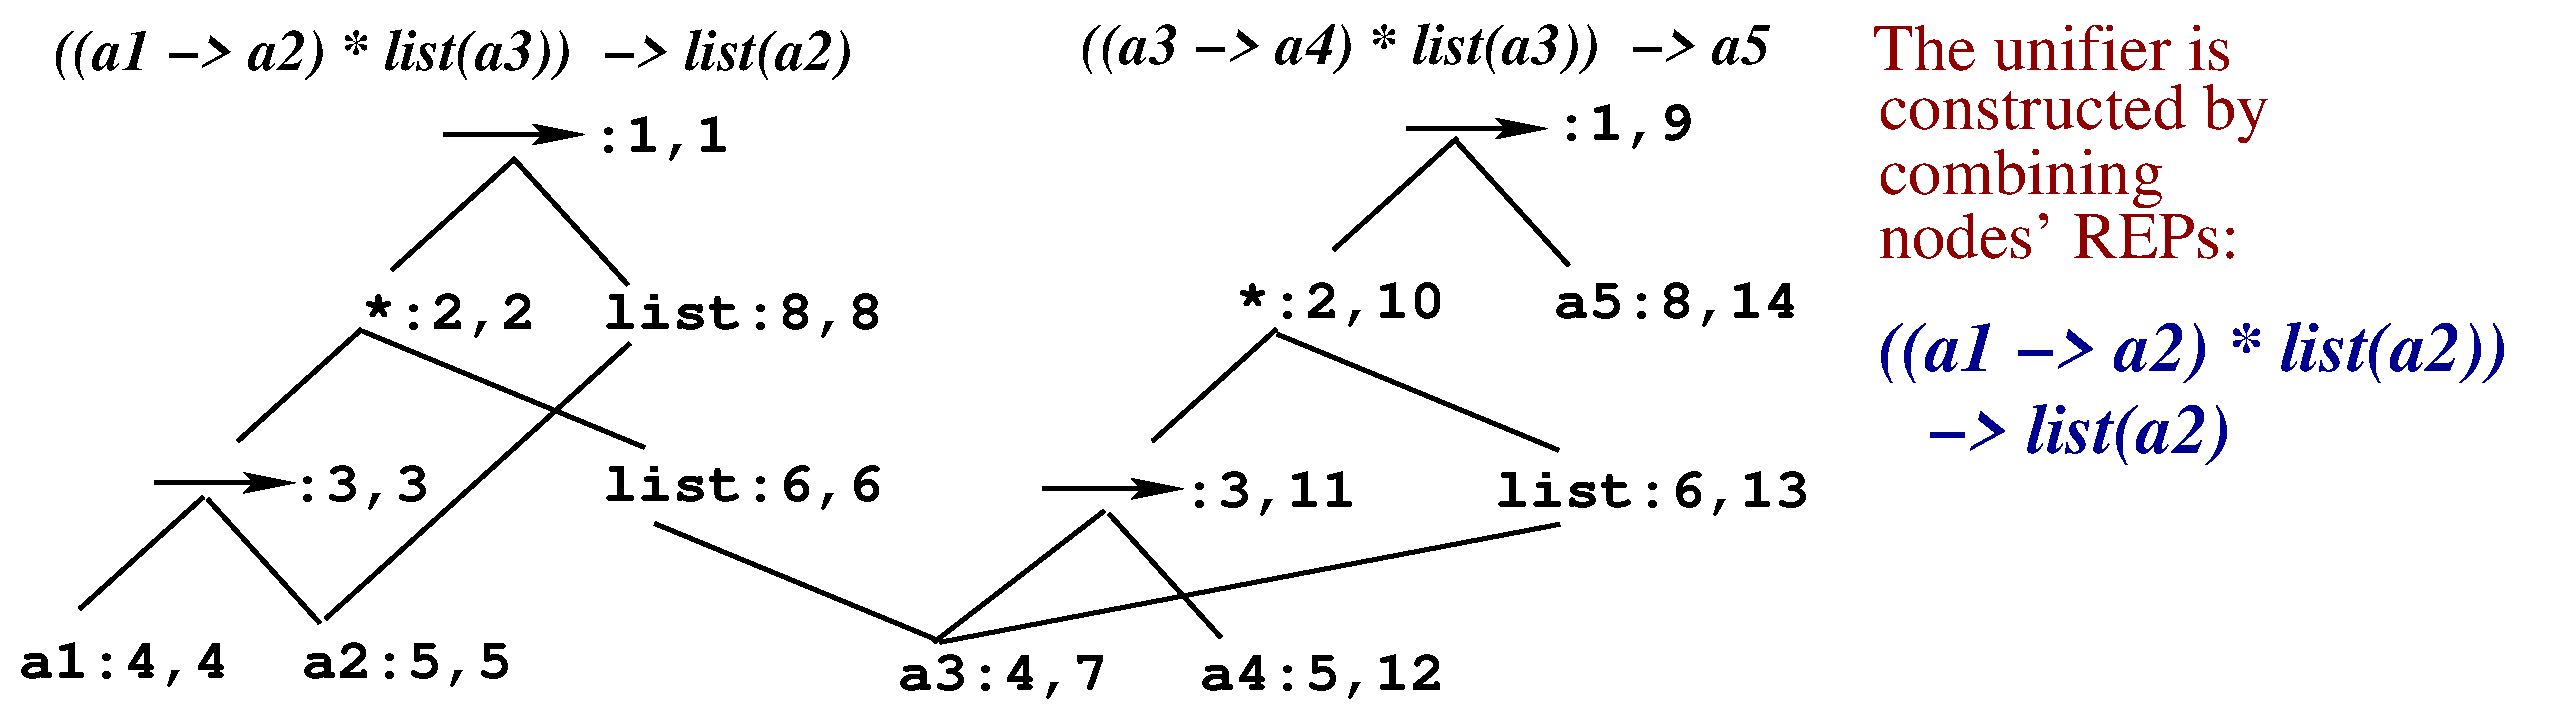
\includegraphics[width=70ex]{Figures/UnificationDone}

\end{frame}
%%%%%%%%%%%%%%%%%%%%%%%%%%%%%%%%%%%%%%%%%%%%%%%%%%%%%%%%%%%%%%%%%%%%%%
%%%%%%%%%%%%%%%%%%%%%%%%%%%%%%%%%%%%%%%%%%%%%%%%%%%%%%%%%%%%%%%%%%%%%%
\section{Type Checker for \textsc{Fasto} With Arrays (SML Code)}

\begin{frame}[fragile]
	\tableofcontents[currentsection]
\end{frame}


\begin{frame}[fragile,t]
   \frametitle{What Changes When Adding Arrays? (part 1)}

\bigskip

Polymorphic Array Constructors and Combinators:

\smallskip

\begin{description}
    \item[replicate:] $\forall~\alpha.~int~*\alpha~\rightarrow~[\alpha]$,\\
                        {\tt replicate(3, a)} $\equiv$ {\tt\{a, a, a\}}.\smallskip
    
    \item[map:] $\forall~\alpha.~\forall~\beta.~(\alpha~\rightarrow~\beta~)~*~[\alpha]~\rightarrow~[\beta]$,\\
                    ${\tt map}(f, \{x_1 ,..,x_n\})~\equiv~\{f(x_1 ),..,f(x_n)\}$\smallskip


    \item[reduce:] $\forall~\alpha.~(\alpha~*~\alpha~\rightarrow~\alpha)~*~\alpha~*~[\alpha]~\rightarrow~\alpha$\\
                        {\tt reduce}$(g,~e,~\{x_1~,..,~x_n\})~\equiv~g(..(g(e,~x_1 )..,~x_n)$

\end{description}

\bigskip

\emp{Question 1: Do we need to implement type inference?}

\bigskip

\emph{Answer 1: No! \textsc{Fasto} supports a fixed set of polymorphic function
whose types are know (or if you like, very simple type inference).} 
\end{frame}


\begin{frame}[fragile,t]
   \frametitle{What Changes When Adding Arrays? (part 1)}

\bigskip

Polymorphic Array Constructors and Combinators:

\smallskip

\begin{description}
    \item[replicate:] $\forall~\alpha.~int~*\alpha~\rightarrow~[\alpha]$,\\
                        {\tt replicate(3, a)} $\equiv$ {\tt\{a, a, a\}}.\smallskip
    
    \item[map:] $\forall~\alpha.~\forall~\beta.~(\alpha~\rightarrow~\beta~)~*~[\alpha]~\rightarrow~[\beta]$,\\
                    ${\tt map}(f, \{x_1 ,..,x_n\})~\equiv~\{f(x_1 ),..,f(x_n)\}$\smallskip


    \item[reduce:] $\forall~\alpha.~(\alpha~*~\alpha~\rightarrow~\alpha)~*~\alpha~*~[\alpha]~\rightarrow~\alpha$\\
                        {\tt reduce}$(g,~e,~\{x_1~,..,~x_n\})~\equiv~g(..(g(e,~x_1 )..,~x_n)$

\end{description}

\bigskip

\emp{Question 2: Assuming type-checking is successful, can we forget the
type of {\tt replicate(3, a)}?}

\bigskip

\emph{Answer 2: No, the type of {\tt a} needs to be remembered for
    machine-code generation, e.g., {\tt a~:~int} {\em vs} {\tt a~:~char}.} \\

Same for array literals, array indexing, map, reduce, etc.
\end{frame}



\begin{frame}[fragile,t]
   \frametitle{What Changes When Adding Arrays? (part 2)}

\bigskip

{\tt map~:~}~$\forall~\alpha.~\forall~\beta.~(\alpha~\rightarrow~\beta~)~*~[\alpha]~\rightarrow~[\beta]$.
        \emp{Type rule for {\tt map(f, x)}:}

\smallskip

\begin{itemize}
    \item compute $t$, the type of {\tt x}, and check that $t~\equiv~[t_{in}]$ for some $t_{in}$.
    \item check that $f~:~t_{in} \rightarrow t_{out}$
    \item if so then {\tt map(f, x)}$~:~[t_{out}]$.
\end{itemize}

\bigskip

\emp{\textsc{AbSyn} representation for {\tt map}:}

\begin{itemize}
    \item {\tt Exp =...| Map of string * Exp * Type * Type * pos},
    \item \alert{Before type checking}, both types are \alert{{\tt UNKNOWN}}. \emph{After:}
    \item the first {\tt Type} is the \emph{input-array element type}, e.g., $t_{in}$,
    \item the second {\tt Type} is the \emph{output-array element type}, e.g., $t_{out}$.
\end{itemize}

\bigskip

\emp{Type checking an expression/program now results in a new exp/prg,
where all the {\tt Type} fields of an expression are filled with known types.}


\end{frame}


\begin{frame}[fragile,t]
    \frametitle{The Gist of Type.sml: Whole Program}



\begin{block}{Type-Checker Entry Point is Function {\tt CheckProgram}}
\begin{colorcode}[fontsize=\scriptsize]
type TabEntry = string * (Type list * Type)
val funTab : TabEntry list ref = ref []

fun checkProgram(funDecs : Fasto.FunDec list) : Fasto.FunDec list =
  let val tab = ("ord",([Fasto.Char (0,0)], Fasto.Int (0,0)))::
                ("chr",([Fasto.Int (0,0)], Fasto.Char (0,0)))::
                (List.map getType funDecs) \emp{(*ftable for declared funs*)}
      \alert{(* Oversimplified: what did I omit to check? *)}

      val () = funTab := tab \emp{(*global,to avoid passing it as param*)}

      \emp{(* type checking each FunDec results in a new FunDec *)}
      \emph{val decorated = List.map checkAndDecorate funDecs}

      (* check main function exists and has type () -> int *) ...
  in \emph{decorated}
  end
\end{colorcode} 
\end{block}

\end{frame}


\begin{frame}[fragile,t]
    \frametitle{The Gist of Type.sml: Type Checking a Function}

\begin{block}{Compute the type of fun's body, check that it matches the result type}
\begin{colorcode}[fontsize=\scriptsize]
fun checkAndDecorate (fid, ret type, args, body, pos) =

  \emp{(* args : (string * Type) list {\em can be used as vtable} *)}
  let val \emph{(body_type, newbody) = expType body args}

  \emp{(* type rule: type of body equals the type of function's result *)}
  in (fid, \emph{typesMatch(body type,ret type)}, args, \emph{newbody}, pos)
  end


fun \emph{typesMatch}( Fasto.Int  p1, Fasto.Int  p2 ) = \emph{Fasto.Int  p1}
  | typesMatch( Fasto.Bool p1, Fasto.Bool p2 ) = \emph{Fasto.Bool p1}
  | typesMatch( Fasto.Char p1, Fasto.Char p2 ) = \emph{Fasto.Char p1}
  | typesMatch( Fasto.Array(t1,p1), Fasto.Array(t2,p2) ) =
                             \emph{Fasto.Array(typesMatch(t1,t2), p1)}
  | typesMatch( t1 , t2 ) = \alert{raise Error("Type error!")}
\end{colorcode} 
\end{block}

\end{frame}




\begin{frame}[fragile,t]
    \frametitle{The Gist of Type.sml: Type Checking an Expression}

\begin{block}{Map Type Rule: the type of array's elems equals the type of fun's arg.}
\begin{colorcode}[fontsize=\scriptsize]
fun \emph{expType} exp vtab = case exp of
    Fasto.Num (n, pos) => (Fasto.Int pos, exp) | ...
  | Fasto.Map (fid, arr, argtype, restype, pos) =>
      let val (arr_type, arr_new) = \emph{expType arr vtab}

          val el_type = case arr_type of
                          Fasto.Array (t,p) => t
                        \alert{| other => raise Error ("Map argument not an array")}

          val (f_arg_type, f_res_type) =
            case SymTab.lookup fid (!funTab) of
              \alert{NONE => raise Error ("Unknown identifier!")}
            | SOME ([a1],res) => (a1,res)
            \alert{| SOME (args,res) => raise Error("Map: not unary fun!")}
          
      in ( Fasto.Array(f_res_type, pos),
           Fasto.Map( fid, \emph{arr_new}, \emp{typesMatch(el_type, f_arg_type)},
                      \emph{f_res_type}, pos ) )
      end
\end{colorcode} 
\end{block}

\end{frame}



%%%%%%%%%%%%%%%%%%%%%%%%%%%%%%%%%%%%%%%%%%%%%%%%%%%%%%%%%%%%%%%%%%%%
%%%%%%%%%%%%%%%%%%%%%%%%%%%%%%%%%%%%%%%%%%%%%%%%%%%%%%%%%%%%%%%%%%%%
%%%%%%%%%%%%%%%%%%%%%%%%%%%%%%%%%%%%%%%%%%%%%%%%%%%%%%%%%%%%%%%%%%%%


\begin{frame}[fragile,t]
    \frametitle{Dead-Function Elimination}

\begin{block}{Partial Pseudocode for {\tt live\_funs}}
\begin{colorcode}[fontsize=\scriptsize]
fun live_funs (
          exp    : Fasto.Exp,
          livefs : string list,
          ftab   : (string * Fasto.FunDec) list
    ) : string list =
  case exp of
\end{colorcode} 
\end{block}

\end{frame}


\begin{frame}[fragile,t]
    \frametitle{Dead-Function Elimination: Recursive-Scan of Expressions}

\begin{block}{Partial Pseudocode for {\tt live\_funs}}
\begin{colorcode}[fontsize=\scriptsize]
fun live_funs (
          exp    : Fasto.Exp,
          livefs : string list,
          ftab   : (string * Fasto.FunDec) list
    ) : string list =
  case exp of
    Plus (e1, e2, p) =>
        \emph{live_funs(e2, live_funs(e1, livefs, ftab), ftab)}

  | ...

\end{colorcode} 
\end{block}

\end{frame}




\begin{frame}[fragile,t]
    \frametitle{Dead-Function Elimination: Scan any Reachable Call}

\begin{block}{Partial Pseudocode for {\tt live\_funs}}
\begin{colorcode}[fontsize=\scriptsize]
fun live_funs (
          exp    : Fasto.Exp,
          livefs : string list,
          ftab   : (string * Fasto.FunDec) list
    ) : string list =
  case exp of
    Plus (e1, e2, p) =>
        \emph{live_funs(e2, live_funs(e1, livefs, ftab), ftab)}

  | ...

  | Map(fid, e, t1, t2, p) =>
        let val \emph{elives = live_funs(e, livefs, ftab)}
        in  \emp{if( fid \mymath{is already in} elives ) then elives}
            \orange{else live_funs( fid's body, fid::elives, ftab )}
        end
\end{colorcode} 
\end{block}

\end{frame}


\end{document}
